\section{Results}
\label{sec:results}

\subsection{Nominal System: Trained Agents (Q2, Q3)}
Table~\ref{tab:main} gives every policy in the nominal system after 100,000 training steps. PPO with the weighted reward misses 2.7\% of critical tasks and 15.4\% of analytics tasks, with an SLA cost of 0.287. This is 10\% above the optimum of 0.261. PPO with the flat reward misses 11.7\% of critical tasks and almost no analytics tasks, with an SLA cost of 0.588, which is 125\% above the optimum and close to the DP policy of the flat reward at 0.510. DQN shows the same pattern, with 0.339 for the weighted reward and 0.550 for the flat reward. Mean critical latency falls from 45.2\,ms to 36.7\,ms for PPO and from 44.8\,ms to 39.3\,ms for DQN. Every PPO and DQN agent sends at least 89\% of tasks to the edge, so none of them avoids misses by hiding tasks in the cloud.

\begin{table*}[t]
\caption{Nominal system after 100,000 training steps. Learning agents: mean over 10 seeds, with a 95\% bootstrap confidence interval for the SLA cost. Rules and DP policies: exact values. All values come from the exact model. Last column: seeds in which the agent has a lower SLA cost than the tuned reservation rule.}
\label{tab:main}
\centering
\footnotesize
\setlength{\tabcolsep}{3.2pt}
\begin{tabular}{@{}lccccccccc@{}}
\toprule
Policy & $v_1$ (\%) & $v_2$ (\%) & All (\%) & Lat. crit (ms) & Lat. ana (ms) & Edge (\%) & SLA cost $J$ & Above optimum & Beats rule \\
\midrule
TABMAINROWS
\bottomrule
\end{tabular}
\end{table*}

Table~\ref{tab:tests} gives the statistics. For PPO and DQN, the weighted agent has fewer critical misses and a lower SLA cost than the flat agent with the same seed in all 10 seeds. The Vargha-Delaney effect size is 0.00 for both, which means that no weighted seed is above any flat seed. All of these differences stay significant after the Holm correction. The corrected reward does not differ from the weighted reward for PPO ($p=1.000$ after correction). Its DP policy is 1.0\% better, which is far below the spread between seeds after 100,000 steps. A2C, now tuned, learns a useful policy, but it is still far from the optimum and its two rewards do not differ in SLA cost.

\begin{table}[t]
\caption{Pairwise tests in the nominal system at 100,000 steps, 10 seeds each. Difference: first minus second reward, in percentage points for miss rates. $A_{12}$: chance that a seed of the first reward has a higher value. $p$: two-sided Mann-Whitney U test, Holm-corrected over all 15 rows. Last column: seeds in which the first reward is lower.}
\label{tab:tests}
\centering
\footnotesize
\setlength{\tabcolsep}{1.8pt}
\begin{tabular}{@{}llcrcrc@{}}
\toprule
Algo & Rewards & Metric & Diff. & $A_{12}$ & $p$ & Lower \\
\midrule
TABTESTROWS
\bottomrule
\end{tabular}
\end{table}

The rules give the reference for Q3. JSQ never uses the cloud, so its queues fill up and it misses 51.8\% of critical tasks. The SLA rule knows the latency model and almost never misses an analytics task, but it misses 11.7\% of critical tasks, with an SLA cost of 0.583. Weighted PPO and weighted DQN beat it in all 10 seeds (sign test, $p=0.002$). The tuned reservation rule sends an analytics task to the edge only when a queue is empty. It misses 1.3\% of critical tasks and 24.1\% of analytics tasks, with an SLA cost of 0.304, which is 16\% above the optimum. Weighted PPO beats it in 9 of 10 seeds ($p=0.021$), and so does corrected PPO. Weighted DQN beats it in 3 of 10 seeds, which is not significant ($p=0.344$). With fair tuning and 100,000 steps, the best learned agent therefore beats a rule that knows the latency model and was tuned on the exact model.

Fig.~\ref{fig:frontier} places every agent against the optimal trade-off. The weighted and corrected PPO agents lie close to the frontier, near the optimum. The flat agents lie near the right end of the frontier, where almost no analytics tasks are missed. They are not bad policies in general. They give the lowest overall miss rate, 6.0\% for flat PPO against 9.0\% for weighted PPO, because the flat reward asks for exactly that, as Proposition 1 shows.

\begin{figure}[t]
\centering
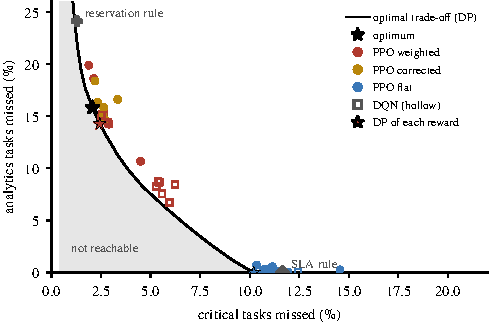
\includegraphics[width=\columnwidth]{fig_frontier_v3.pdf}
\caption{Trade-off between critical and analytics misses in the nominal system. The black line is the optimal trade-off from DP, and no policy can reach the gray area. Filled circles: PPO agents after 100,000 steps, one per seed. Hollow squares: DQN agents. Stars: the optimum and the DP policy of each reward.}
\label{fig:frontier}
\end{figure}

\subsection{Learning Curves and Training Budget}
Fig.~\ref{fig:curves} shows the SLA cost during training, scored exactly every 5,000 steps, over 10 seeds. Weighted PPO first reaches the level of the tuned reservation rule at 40,000 steps and stays at or below it for the rest of training, within 0.001. Corrected PPO reaches it at 50,000 steps and then moves around it. Flat PPO reaches about 0.57 after 20,000 steps and does not improve further. DQN with the scaled weighted reward reaches about 0.33 after 25,000 steps and stays between 0.31 and 0.35, so the instability of the conference settings is gone. A2C improves slowly and is still far from the other two at 100,000 steps. With the settings of the conference version and 20,000 steps, the reservation rule beat every agent in every seed. Both the tuning and the longer training are needed for the learned agents to reach the level of a tuned rule.

\begin{figure*}[t]
\centering
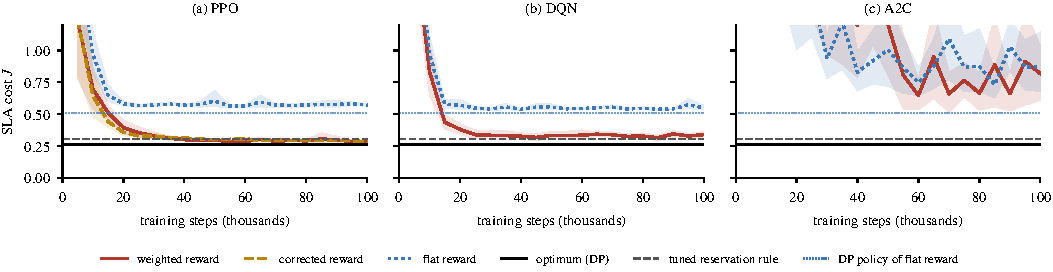
\includegraphics[width=\textwidth]{fig_curves_v3.pdf}
\caption{SLA cost during training in the nominal system, scored by the exact model every 5,000 steps. Mean over 10 seeds with 95\% bootstrap confidence interval. PPO updates in blocks of 1,024 steps, so its final policies in Table~\ref{tab:main} are taken after 100,352 steps, one update after the last point of the curve. Black line: optimum. Gray dashed line: tuned reservation rule. Thin dotted line: DP policy of the flat reward.}
\label{fig:curves}
\end{figure*}

\subsection{Published Reward Designs (Q3)}
Table~\ref{tab:pub} gives the design of Yamsani and Chenna Reddy \cite{yamsani2026} rebuilt in the nominal system. With risk features, action pruning and adaptive tiers, PPO reaches an SLA cost of 0.368 with a step size of 0.001 and 0.418 with 0.01, which is 41\% and 60\% above the optimum. With adaptive tiers alone it reaches 0.414. All three versions are better than the flat reward of Nieto et al. \cite{nieto2024} in every seed, and worse than the fixed weighted reward in every seed (Mann-Whitney, $p<0.001$ for each comparison). None of them beats the tuned reservation rule in any seed.

\begin{table}[t]
\caption{Rebuilt design of Yamsani and Chenna Reddy \cite{yamsani2026} in the nominal system, PPO, 100,000 steps, 10 seeds. Penalties: mean penalty of the critical and the analytics tier at the end of training. The full design is scored by 500 simulated episodes, because its state has risk features (standard error of each SLA cost below 0.01). All other rows are exact.}
\label{tab:pub}
\centering
\footnotesize
\setlength{\tabcolsep}{2pt}
\begin{tabular}{@{}lccccc@{}}
\toprule
Variant & $\eta$ & SLA cost $J$ & Above & $v_1$ (\%) & Penalties \\
\midrule
TABPUBROWS
\midrule
PPO weighted & & PPOWCI & PPOWGAP & PPOWCRIT & 10, 2 \\
PPO flat & & PPOFCI & PPOFGAP & PPOFCRIT & 6, 6 \\
\bottomrule
\end{tabular}
\end{table}

Proposition 1 explains the result. The design raises the penalty of a tier whenever its recent miss rate is above the target of 5\%. In this system the optimum misses 15.8\% of analytics tasks, so the analytics target cannot be met together with a low critical miss rate. Both penalties keep growing, and the analytics penalty grows faster relative to its start. After training the penalties are 11.1 and 4.7 with the smaller step size, and 30.0 and 14.1 with the larger one. With the bonus of 1, they act as a ratio of about 2:1 instead of the operator's 5:1, so the agent moves toward the class-blind policy. Adaptive penalties work well when every target is reachable \cite{altman1999,tessler2019}. When the targets are set without knowing what is possible, they can undo the per-class weighting that the tiers were meant to provide. The exact model shows which targets are reachable, through the Pareto frontier of Fig.~\ref{fig:frontier}.

\subsection{Larger Systems (Q4)}
Table~\ref{tab:scen} and Fig.~\ref{fig:scen} give the three larger systems. PPO was tuned again for each system with the same protocol, now with the three best PPO settings of the nominal tuning, two tuning seeds and the full budget. The default setting was chosen for Hetero3 and Large4-3C, and the nominal setting for Hetero3-3C. The rules are much further from the optimum here than in the nominal system. The tuned reservation rule is 32\% to 89\% above the optimum, and the rule with node sets 21\% to 31\%.

\begin{table}[t]
\caption{Larger systems. PPO tuned for each system, mean over 10 seeds with 95\% bootstrap interval. Rules: exact. Miss rates per class in \%. Last column: seeds in which PPO beats the node-set rule.}
\label{tab:scen}
\centering
\footnotesize
\setlength{\tabcolsep}{1.6pt}
\begin{tabular}{@{}lcccc@{}}
\toprule
Policy & SLA cost $J$ & Above opt. & $v_c$ (\%) & Beats \\
\midrule
TABSCENROWS
\bottomrule
\end{tabular}
\end{table}

\begin{figure*}[t]
\centering
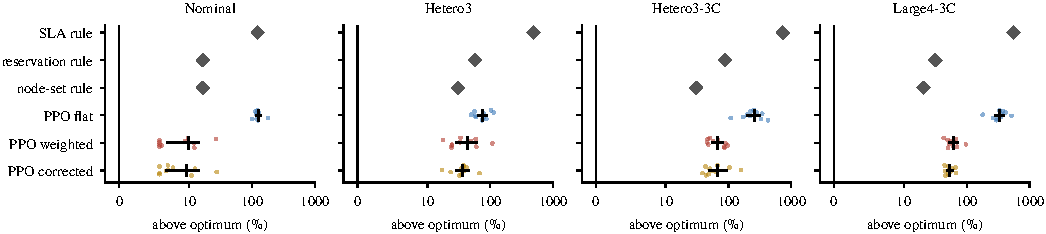
\includegraphics[width=\textwidth]{fig_scenarios_v3.pdf}
\caption{Distance of every policy to the optimum of its system, in percent on a scale that is linear below 10\% and logarithmic above. Diamonds: rules, exact. Dots: PPO agents, one per seed, with the mean and its 95\% bootstrap interval in black. Nominal system after 100,000 steps, Hetero3 and Hetero3-3C after 100,000 steps, Large4-3C after 200,000 steps.}
\label{fig:scen}
\end{figure*}

The effect of the reward carries over to every larger system. The weighted reward lowers the SLA cost of PPO against the flat reward in Hetero3 from 0.158 to 0.129, in Hetero3-3C from 0.298 to 0.140 and in Large4-3C from 0.340 to 0.125. All three differences are significant after the Holm correction ($p \le 0.036$), and in the three-class systems every weighted seed is below every flat seed. The corrected reward gives 0.123, 0.140 and 0.120, which does not differ significantly from the weighted reward in any system. Its exact advantage of up to 10\% in the DP policies is therefore smaller than what PPO reaches in practice.

The trained agents are still far from the optimum, 36\% to 67\% above it for the weighted and corrected rewards. They beat the SLA rule in every seed of every system. Against the tuned reservation rule the picture depends on the system. Corrected PPO beats it in 9 of 10 seeds in Hetero3 ($p=0.021$), weighted and corrected PPO beat it in 8 of 10 seeds in Hetero3-3C ($p=0.109$), and no agent beats it in Large4-3C. The rule with node sets is better than every agent in Hetero3-3C and Large4-3C, and better than most seeds in Hetero3. In these systems a rule that knows the latency model and is tuned on the exact model is still the stronger choice. The agents learn from rewards alone and reach this level without any model, but the exact benchmark shows that they leave a large part of the possible gain unused.

With the nominal PPO setting instead of the setting tuned per system, the weighted reward reaches 0.134, 0.140 and 0.162, and the corrected reward 0.117, 0.140 and 0.133. The order of the rewards is the same. The setting matters most in Large4-3C, where the default setting is more stable across seeds and lowers the cost of weighted PPO from 0.162 to 0.125. In Hetero3 the nominal setting is slightly better for the corrected reward, which then beats the node-set rule in 7 of 10 seeds.

\subsection{Changes of the System (Q5)}
Table~\ref{tab:shift} and Fig.~\ref{fig:shift} give the five changes of the nominal system. Every value is the distance to the optimum of the changed system. The SLA rule with the nominal latency model is 106\% to 239\% above the optimum. The tuned reservation rule keeps its nominal threshold, which sends an analytics task to the edge only when a queue is empty. Tuning it again with the true model of the changed system picks the same threshold in all five cases, so the rule loses nothing from the change and stays 6\% to 16\% above the optimum. This matches the structure of the optimal policy for one pool of servers \cite{miller1969}, which does not depend on the exact speeds.

\begin{table*}[t]
\caption{Changes of the nominal system. Distance of the SLA cost to the optimum of the changed system, exact. Nominal: policy or threshold of the nominal system used unchanged. Re-tuned: thresholds chosen again on the exact model of the changed system. Fine-tuned: nominal PPO network trained for another 25,000 steps in the changed system. PPO values are means over 10 seeds.}
\label{tab:shift}
\centering
\footnotesize
\setlength{\tabcolsep}{4pt}
\begin{tabular}{@{}lcccccccc@{}}
\toprule
 & & SLA rule & \multicolumn{2}{c}{Reservation rule} & \multicolumn{2}{c}{PPO weighted} & \multicolumn{2}{c}{PPO flat} \\
\cmidrule(lr){4-5} \cmidrule(lr){6-7} \cmidrule(l){8-9}
Change & Optimum & nominal model & nominal & re-tuned & nominal & fine-tuned & nominal & fine-tuned \\
\midrule
TABSHIFTROWS
\bottomrule
\end{tabular}
\end{table*}

\begin{figure}[t]
\centering
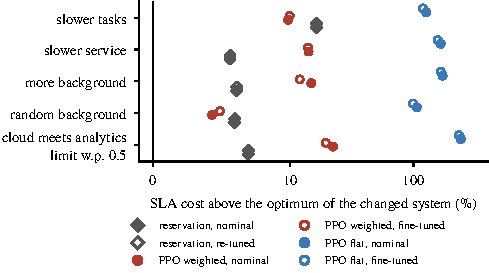
\includegraphics[width=\columnwidth]{fig_shift_v3.pdf}
\caption{Distance to the optimum of the changed system for the reservation rule and PPO, on a scale that is linear below 10\% and logarithmic above. Filled markers: nominal rule or policy used unchanged. Hollow markers: re-tuned rule or fine-tuned agent. PPO values are means over 10 seeds.}
\label{fig:shift}
\end{figure}

The trained PPO agents also keep most of their quality without any new training. Weighted PPO with its nominal policy is 4\% to 22\% above the new optimum. It beats the unchanged reservation rule in 9 of 10 seeds when tasks get slower and when the background becomes random, and loses to it under the other three changes. Another 25,000 steps of training in the changed system move the weighted agents by at most 3 percentage points, to between 5\% and 19\% above the optimum. The order of the rewards does not change. Flat PPO is 99\% to 242\% above the optimum under every change, with or without fine-tuning. In these changes the best structure stays the same, which is to keep the edge free for critical tasks, so a policy that has learned this structure keeps working.

\subsection{Sensitivity at a Short Budget}
The conference version also changed the penalty ratio, the load, the class mix and the learning rate, with PPO in its default setting, 20,000 steps and 10 seeds (5 for the learning rate). These results are scored with the exact model and summarized here. Fig.~\ref{fig:sweeps}(a) changes the penalty ratio with the average penalty fixed at 6. Critical misses fall from 13.6\% at 6:6 to 5.1\% at 11:1, and analytics misses rise from 0.8\% to 19.5\%. Fig.~\ref{fig:sweeps}(b) changes the service probability $d$ from 0.9 to 0.5, which moves the offered load from 0.67 to 1.2. With spare capacity, at a load of 0.67 and 0.75, both rewards miss almost no tasks and do not differ ($p=0.940$ and $p=0.853$). At a load of 1.2 the weighted reward halves the SLA cost of the flat reward, 1.099 against 2.112 ($p<0.001$). The per-class penalty matters only when the classes compete for the edge. Fig.~\ref{fig:sweeps}(c) changes the share of critical tasks. At 30\% critical tasks the weighted reward lowers the SLA cost from 0.785 to 0.537 ($p=0.005$). At 70\% it lowers the mean from 0.894 to 0.633, which is not significant ($p=0.105$). A learning rate of $10^{-4}$ does not learn within 20,000 steps with either reward. At $3\times10^{-4}$ and $10^{-3}$ the weighted reward has the lower SLA cost.

\begin{figure*}[t]
\centering
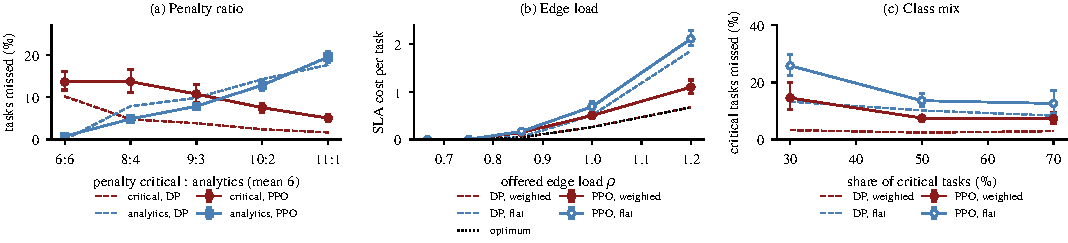
\includegraphics[width=\textwidth]{fig_sweeps.pdf}
\caption{Sensitivity of PPO with the conference setting at 20,000 steps, mean over 10 seeds with 95\% bootstrap confidence interval, against the DP policy for the same reward (dashed). (a) Penalty ratio with the average penalty fixed at 6. (b) Offered edge load $\rho$, changed through the service probability $d$. (c) Share of critical tasks, with the flat penalty matched to the mix by Eq.~\eqref{eq:flat}.}
\label{fig:sweeps}
\end{figure*}

\subsection{Short Test Sets}
Every agent was also simulated on 100 held-out episodes. Short and fixed test sets can move results noticeably. Table~\ref{tab:protocol} shows the critical miss rate of three fixed policies, exact and simulated. With the 20 episodes used in the conference version, the SLA rule shows 10.67\% critical misses against an exact 11.65\%. With 3,000 episodes the difference falls below 0.1 percentage points. A shift of one percentage point is as large as some of the differences that offloading papers report, which is why every number in this paper comes from the exact model.

\begin{table}[t]
\caption{Critical miss rate (\%) of three fixed policies in the nominal system, exact and simulated on fixed test sets of different size.}
\label{tab:protocol}
\centering
\footnotesize
\setlength{\tabcolsep}{4pt}
\begin{tabular}{@{}lcccc@{}}
\toprule
Policy & Exact & 20 episodes & 100 episodes & 3,000 episodes \\
\midrule
SLA rule & 11.65 & 10.67 & 12.59 & 11.72 \\
Reservation rule & 1.26 & 1.01 & 1.39 & 1.29 \\
Optimum (DP) & 2.06 & 1.71 & 2.25 & 2.09 \\
\bottomrule
\end{tabular}
\end{table}
